\chapter{Trabalhos Analisados}
\label{cap:trabalhos-analisados}

Esse capítulo tem como objetivo destacar as principais pesquisas recentemente
realizadas com o objetivo de expandir as abstrações de processos. Para a
seleção dos trabalhos aqui apresentados, o autor levou em consideração os
seguintes aspectos: quantidade de citações dos trabalhos, implementação
funcional e pesquisas que tenham a abstração de processos como objeto de
estudo. Por uma questão de organização, esse trabalho considerou três tipos de
implementação funcional: \textit{Implementação Estrutural Leve, Implementação
Estrutural Pesada e Implementação Independente}.

Chamamos de \boldAndIndex{Implementação estrutural leve} toda proposta que não
altera diretamente o núcleo do SO. Isso faz com que a proposta tenha uma chance
maior de ser incorporada em um SO de produção e, ao mesmo tempo, gera pouco
impacto geral no SO. Normalmente, implementações leves utilizam artifícios de
\emph{device drivers} (Veja \ref{sec:dd}), o que torna simples de desenvolver e
testar novas propostas.

As \boldAndIndex{Implementações Estruturais Pesadas} são aquelas que alteram
diretamente o núcleo do SO. Essa abordagem traz vantagens e desvantagens que
devem ser consideradas antes de serem adotadas. Por um lado, alterações diretas
no núcleo são mais flexíveis em termos de possibilidade de acesso aos recursos
disponíveis do SO. Por outro lado, alterações no núcleo são arriscadas, uma vez
que podem afetar toda a estabilidade do sistema, e são extremamente complexas
de serem feitas, uma vez que demandam profundo conhecimento do SO em questão.

As \boldAndIndex{Implementações Independentes} são aquelas que se propõem a
criar um SO totalmente novo, visando demonstrar um ou mais conceitos. Essas
abordagens têm poucas chances de serem adotadas diretamente, contudo apresentam
conceitos e ideias que podem ser interessantes para serem estendidas para SOs
atuais. Nessa dissertação trataremos especificamente do Exokernel devido ao seu
grande impacto (Seção~\ref{sec:exokernel}), contudo, trabalhos como o
\emph{Singularity}~\citep{aiken} e o \emph{Corey}~\citep{corey} também
influenciaram essa dissertação.

Em resumo, esse capítulo busca fornecer uma visão geral sobre o estado da arte
das abstrações de processos. Além disto, essa seção visa proporciona as bases
para a discussão apresentada no Capítulo
\ref{cap:analise-sobre-abstracoes-de-processos}, tema central desse trabalho.
Os trabalhos apresentados adiante, se encaixam em pelo menos uma das
características de implementação discutidas acima.

\section{Dune}
\label{sec:dune}

Como mostrado na Seção \ref{sec:virtualizacao}, o conceito de virtualização já
é amplamente conhecido e adotado pela indústria; dentre os recentes avanços,
destaca-se a virtualização via hardware proporcionada pelos processadores
modernos. O mecanismo de virtualização é normalmente utilizado fornecendo
abstrações para a criação de máquinas virtuais. Com esse conceito em mente,
\citet{belay} decidiram dar outra utilidade para esses recursos de hardware:
fornecer características adicionais para processos ao invés de máquinas
virtuais.

Os autores defendem que uma ampla variedade de aplicações pode tirar proveito
do acesso a certos recursos que são apenas disponíveis ao kernel. Dentre as
aplicações que podem comprovadamente ganhar algum desempenho ao obter acesso
direto ao hardware, destacam-se:

\begin{itemize}
  \item \textbf{Coletor de Lixo (\emph{Garbage Collection -- GC})}: O GC pode ganhar desempenho caso
        tenha como controlar diretamente o hardware de paginação, como
        \citet{pauseless} demostraram em seu trabalho;
  \item \textbf{Migração de Processos}: Programas no espaço de usuário podem tirar
        proveito do acesso direto às faltas de páginas e chamadas de sistemas para
        implementar novas técnicas de migração de processos.
\end{itemize}

Não obstante, fornecer o acesso direto aos recursos de hardware de forma segura
e gerenciável não é uma tarefa trivial, uma vez que requer mudanças na forma
como o espaço de usuário e o espaço do Kernel interagem. Além disso, alterações
no Kernel são consideradas invasivas e perigosas, uma vez que uma modificação
feita de forma errada pode comprometer toda a estabilidade do sistema. Outra
alternativa para dar acesso de hardware para aplicações é por meio de execução
em uma máquina virtual assim uma aplicação consegue acesso seguro aos recursos
de hardware através da interface de virtualização. Uma desvantagem desta
abordagem é que ela tem pouca integração com o SO da máquina \emph{host}, o que
impede o processo de obter ganhos de desempenho.

\citet{belay} oferecem uma alternativa que consiste em utilizar a abstração de
virtualização disponível nos processadores modernos de forma a fornecer um novo
tipo de processo que executa no chamado \emph{Dune Mode} (modo Dune). Tal modo
é um estado irreversível no qual o processo indica explicitamente que quer
entrar; nesse modo, o processo passa a ter acesso direto, por meio dos recursos
de virtualização, a modos de operação com maior privilégio, registradores de
memória virtual, tabelas de páginas, interrupções, exceções e vetores de
chamada de sistema. Para auxiliar a aplicação no espaço de usuário a interagir
com tais recursos, os autores criaram uma biblioteca chamada \emph{libDune} que
dá apoio à utilização das novas funcionalidades.

Dentre as vantagens que essa pesquisa promete, destacam-se o fato de que o modo
Dune mantém a compatibilidade com os processos, i.e., a aplicação não precisa
ser fortemente modificada. Quando um processo faz uma chamada de sistema, ele
dispara uma instrução chamada \texttt{SYSCALL}, contudo, aplicações que
manipulam recursos de virtualização utilizam a \texttt{VMCALL} para manter o
isolamento. O Dune utiliza o recurso do \texttt{VMCALL} para tirar o máximo
de isolamento fornecido pelo hardware de virtualização. Além disso, devido ao
fato de que o Dune não tem por objetivo fornecer máquinas virtuais, ele
consegue ser mais simples e rápido. As aplicações que se adequam ao uso desse
modelo podem obter melhorias de desempenho e isolamento, como veremos adiante.

Para implementar o Dune, os pesquisadores utilizaram processadores Intel com
suporte para a tecnologia VT-x e parte do código do KVM já disponível no Kernel
Linux. Na Seção~\ref{sec:vtx} apresentamos o VT-x e algumas instruções
importantes para o contexto da virtualização, agora introduzimos os três tipos
de instruções privilegiadas que o Dune fornece para os processos:

\begin{itemize}
	\item \textbf{Exceções}:  As instruções \texttt{LIDT, LTR, IRET, STI e CLI} são
        expostas diretamente para os processos. Note que emulação, depuração e
        rastreamento de desempenho são atividades que podem tirar proveito
        desta característica, uma vez que o Dune pode reduzir consideravelmente
        a sobrecarga em entregar exceções. Isso se deve ao fato que o Dune
        consegue entregar exceções diretamente para o hardware de forma segura
        (encapsulado pelo hardware de virtualização);
  \item \textbf{Memória Virtual}: As instruções \texttt{MOV CRn, INVLPG} e
        \texttt{INVPCID} são oferecidas para o processo Dune. O acesso
        flexível à memória virtual pode ser benéfico para aplicações que fazem
        \emph{checkpointing}, GC, compressão de dados nas páginas e utilizam memória
        compartilhada distribuída. O Dune traz melhorias para o acesso à
        memória virtual expondo as entradas da tabela de páginas para as
        aplicações. Isso permite que elas controlem a tradução de endereços,
        as permissões de acesso, bits globais e que elas modifiquem/acessem as páginas com
        simples referências. Por fim, o Dune também dá a habilidade de
        controlar as invalidações da TLB manualmente, o que pode ser vantajoso
        para alguns tipos de aplicações;
  \item \textbf{Modos privilegiados}: As instruções \texttt{SYSRET, SYSEXIT, IRET}
        permitem que o Dune exponha os modos privilegiados de
        forma segura. O Dune expõe esse modos de forma eficiente e segura por
        que o VMX non-root mantém o seu próprio conjunto de anéis privilegiados
        (Veja \ref{sec:vtx}).
\end{itemize}

A Figura \ref{fig:dune_architecture} ilustra a arquitetura do Dune. O Dune
estende o Kernel como um módulo que habilita o VT-x, colocando-o no
modo VMX root. Assim, processos usando Dune têm acesso seguro e garantido para
hardware privilegiado utilizando o modo VMX non-root. O módulo Dune intercepta
transições para o {VM exits} (Seção~\ref{sec:vtx}), o único motivo para o
processo acessar o kernel e realizar qualquer ação. Repare que o Dune é
aplicado de forma seletiva aos processos que de fato precisam dele, o que
significa que um processo que não usa o Dune não é afetado. A transição de um
processo normal para o modo Dune ocorre por meio de uma chamada de
\texttt{ioctl} no dispositivo \texttt{/dev/dune} e, ao entrar nesse modo, o
processo não pode retornar ao modo anterior. Sempre que um processo Dune faz um
\texttt{fork()}, o processo filho não inicia em modo Dune, contudo pode
reentrar caso queira.

\begin{figure}[!h]
  \centering
  \includegraphics[width=0.6\textwidth]{dune_architecture} 
	\caption[Arquitetura do Dune]{Arquitetura do Dune~\citep{belay}}
  \label{fig:dune_architecture}
\end{figure}

Na Seção \ref{sec:virtualizacao}, apresentamos as principais propriedades dos VMMs.
Com o objetivo de deixar claras as diferenças entre o VMM e as características
de hardware expostas pelo Dune, destacamos as principais diferenças:

\begin{itemize}
  \item No Dune, o mecanismo de \textit{hypercall} invoca
        \textit{system calls} comuns do Linux;
  \item Apenas características de hardware que podem ser acessadas diretamente,
        sem a intervenção do VMM, são disponíveis para a aplicação. Nos casos em
        que não é possível executar uma dada operação, Dune devolve o controle
        para o SO;
  \item Podemos reduzir as diferenças de estados entre o \textit{guest} e o \textit{host}, uma
        vez que processos usando Dune têm uma interface próxima da de hardware;
  \item No Dune, é preciso configurar o EPT para refletir o endereço do espaço
        de usuário.
\end{itemize}

\section{Shreds}

Existe uma categoria de ataques chamada ``abusos intra-processos de conteúdo
de memória'', na qual o invasor busca acessar determinado tipo de conteúdo
sensível na memória (p.ex., dados secretos) ou uma região de código crítica
(p.ex., funções privilegiadas) \citep{shreds}. O roubo desse tipo de dados
acontece por meio da introdução de algum código injetado ou por meio de alguma
biblioteca maliciosa que permite acessar alguma região da memória não protegida
da vítima. Note que bibliotecas maliciosas são especialmente perigosas, uma vez
que elas podem executar funções privilegiadas que são de fato parte do
processo como, por exemplo, a função \texttt{dlopen}. Por fim, se o atacante
conseguir o acesso a memória, ele pode ler todos os dados buscando por outras
informações.

\citet{shreds} defendem que o problema de segurança referente aos ataques
intra-processos decorrem da falta de controle fino e eficiente do conteúdo
sensível da memória; além disso, eles argumentam que seria benéfico se tais
funcionalidades fossem disponibilizadas para os programadores. Para resolver tal
problema, os autores apresentam uma nova abstração de processos que cria uma
nova unidade de execução chamada \emph{shred}, que tem associado a si um
fragmento de memória protegida denominado \emph{shred-private pool
(s-pool)}. O tamanho do segmento de memória criado é variável,
dependendo da necessidade da aplicação. Além disso ele se comporta de forma a
existir apenas durante o momento em que é necessário para um pedaço da
aplicação. A implementação do \emph{shreds} é baseada em três pilares: uma API
para o usuário conseguir utilizar facilmente as funcionalidade oferecidas, um
conjunto de ferramentas de compilação que verifica a correta utilização dos
\emph{shreds} (\emph{S-compiler}) e um módulo Linux que faz o gerenciamento da
memória (\emph{S-driver}).

\emph{Shreds} foi projetado buscando três propriedades que visam garantir
segurança:

\begin{itemize}
  \item \textbf{Acesso exclusivo para s-pool:} Um \emph{s-pool} só é acessível
        para o \emph{shred} associado a ele;
  \item \textbf{controle de vazamentos na entrada e saída:} Dados carregados em um
        \emph{s-pool} não podem ser copiados ou exportado sem que seja
        executada uma operação de limpeza;
  \item \textbf{Execuções não desviáveis:} O fluxo de execução não pode ser
        alterado para fora do \emph{shred}.
\end{itemize}

Para melhor entender o comportamento dos \emph{shreds}, veja a Figura
\ref{fig:shreds}, ilustrando uma aplicação que lida com uma senha (dado
sensível) e o código que manipula tal dado. A aplicação possui uma \emph{thread} que
comporta-se da forma padrão, contudo, ao ter que lidar com um dado sensível, ela
faz uma chamada para uma função da API fornecida pelo \emph{shred},
\texttt{shred\_enter()}. Ao realizar a chamada para essa função, o fluxo de
execução entra em um modo seguro em que o \emph{shreds} gerencia o acesso à
memória e garante que os dados são isolados do restante da aplicação. Por fim,
após realizar a operação na região protegida, a aplicação do usuário chama
\texttt{shred\_exit()}. Para utilizar a proposta dos autores, é preciso alterar
as aplicações alvo.

\begin{figure}[!h]
  \centering
  \includegraphics[width=0.6\textwidth]{shreds} 
  \caption{Funcionamento geral do shreds}
  \label{fig:shreds}
\end{figure}

A API fornecida pelo \emph{shreds} consiste em apenas quatro funções:

\begin{itemize}
  \item \texttt{shred\_enter()}: Muda o fluxo de execução da \emph{thread} atual e
        cria uma cópia da pilha atual do processo em uma região de memória
        segura (\emph{pool});
  \item \texttt{shred\_exit()}: Suspende o \emph{shred} chamado, revoga as permissões
        de acesso da \emph{thread} atual sobre o \textit{s-pool} e recupera a pilha de execução
        original;
  \item \texttt{spool\_alloc()}: Aloca memória para o \emph{s-pool} associado à
        \emph{thread};
  \item \texttt{spool\_free()}: Apaga a memória alocada.
\end{itemize}

Para garantir que as regras de utilização da API sejam seguidas, o
\emph{S-compiler} realiza verificações e instrumentações para evitar falhas que
abram brechas de segurança.

Para este trabalho, a parte mais importante do \emph{shred} é o \emph{S-driver},
que consiste em um módulo do Linux responsável por gerir os \emph{shreds} e
\emph{s-pools}. A implementação dessa técnica é baseada em domínios de memória
do ARM (Seção \ref{sec:outros_mecanismos_memoria}). Contudo, dado que essa
tecnologia não foi projetada para os propósitos sugeridos pelo \emph{shreds},
ela apresenta duas limitações:

\begin{itemize}
  \item O ARM fornece apenas 16 domínios, o que impede que se crie um domínio
        para cada \emph{s-pool}, uma vez que seu número pode crescer de forma
        indeterminada;
  \item O controle de acesso à memória é extremamente limitado.
\end{itemize}

A solução adotada pelos autores foi implementar um mecanismo que multiplexa os
domínios e introduz identidades dentro da lógica de acesso. Para permitir que
uma aplicação tenha várias \emph{shreds}, o \emph{S-driver} utiliza os domínios
de forma temporária, rotacionando as identidades de segurança para o
\emph{s-pool}. Toda vez que uma \emph{shreds} inicia ou retoma a sua execução
em uma $CPU_i$ o \emph{S-driver} atribui um \emph{s-pool} associado a um
domínio $Dom_i$. Isso faz com que uma \emph{shred} consiga acessar o seu
\emph{s-pool} enquanto outras \emph{threads} concorrentes não. Quando o
\emph{shred} finaliza ou tem a sua execução parada em favor de outro
processo, o \emph{S-driver} muda o domínio, prevenindo que outro processo
consiga acessar a região de memória. Note que o \emph{driver} permite ou
rejeita o acesso a um \emph{s-pool} baseado na CPU; isso faz com que, mesmo que
um código malicioso consiga executar em paralelo com o \emph{shred}, ele não
consiga ter acesso ao \emph{s-pool} sem que seja disparada uma falha de
domínio.

Uma das funcionalidades fornecidas pelo \emph{shread} é a habilidade de
permitir fazer cópias de dados para regiões de memória não protegidas de forma segura
(p.ex., atribuir dados de um \emph{s-pool} para uma variável local). Note que,
para realizar tal procedimento, é preciso acessar uma pilha regular que pode ter
sido atacada e conter um código mal-intencionado, o que violaria toda proteção
fornecida pelo \emph{s-compiler} e \emph{S-driver}. Para prevenir que dados
sejam vazados via pilha, o \emph{S-driver} cria uma pilha segura para cada
\emph{shred} alocada partindo do \emph{s-pool} associado a si.

\section{Wedge}

Existe um princípio chamado de \emph{``Princípio do Menor Privilégio''} que diz:

\begin{quote}
O princípio do menor privilégio implica dividir o código em compartimentos,
cada um dos quais executa com os privilégios mínimos necessários para completar
sua tarefa. Essa abordagem não apenas limita o dano que um ataque pode causar,
mas também pode evitar que os \emph{bugs} vazem acidentalmente informações
confidenciais.
\end{quote}

Apesar desse princípio ter sido apresentado em 1975 e ser amplamente aceito,
nota-se que várias aplicações que tem acesso à Internet (um ponto de acesso
para o mundo) não buscam atender a esse fundamento e acabam abrindo
potenciais pontes de vazamento de dados ou falhas de segurança. Alguns
pesquisadores defendem que esse problema surge do fato de que os SO atuais
garantem privilégios por padrão. Isso significa que impor limites requer mais
esforço por parte do programador e também é propenso a erros.

A chamada de sistema \texttt{fork()} ilustra a característica de garantir
privilégios por padrão. Quando o processo pai cria um filho, este inicia como uma
cópia praticamente exata do pai. Se o programador desejar restringir o nível de
acesso do processo filho, é preciso realizar uma série de operações manuais que
não garantem que nenhum aspecto tenha sido ignorado.

\citet{wedge} buscaram resolver tal problema mudando o princípio atual, de
garantir privilégio por padrão, para negar privilégios por padrão. Nessa
abordagem, o programador deve indicar explicitamente que deseja garantir
permissões adicionais. Os autores alteraram o GNU/Linux para que ele
suportasse a remoção de permissões por padrão e chamaram o modelo proposto por
eles de \emph{Wedge}. \emph{Wedge} fornece um conjunto de primitivas de
programação para permitir criar componentes com semântica de negação de permissões
por padrão, tornando o acesso mais restrito. Para isso, \emph{Wedge} oferece
um esquema simples e flexível de marcação (\emph{tagging}) das permissões de
acesso à memória, permitindo que o programador aloque objetos na memória de
acordo com essa informação.

\emph{Wedge} permite que o programador crie um número arbitrário de
componentes, cada um sem privilégios por padrão, mas existem mecanismos que
permitem o controle fino. Neste sentido, \emph{Wedge} busca se assemelhar às
primitivas atuais para facilitar a sua adoção e para que seja simples a
introdução delas em aplicações legadas. A proposta é constituída de três
primitivas: \emph{Sthread}, \emph{Tagged Memory} e \emph{callgates}. O
acesso a todas essas primitivas é feito via chamadas de sistema.

Uma \emph{Sthread} pode ser comparada com uma \emph{thread} fornecida pela biblioteca
\textit{pthread}, definindo um compartimento dentro de uma
aplicação. O programador pode então atribuir permissão de acesso para a memória
e outros recursos por meio dessas \emph{sthreads}. Elas consistem de uma
\emph{thread} de controle e políticas de segurança associadas, que especificam:

\begin{itemize}
	\item As marcações de memória que a \emph{sthread} pode acessar e a permissão
				sobre cada cada uma (leitura, leitura-escrita e \textit{copy-on-write});
	\item Os descritores de arquivo que a \emph{sthread} pode acessar e as
				permissões sobre cada (leitura, escrita, leitura-escrita);
	\item Os \emph{callgates} que a \emph{sthread} pode chamar;
	\item O \emph{Unix user id}, o diretório raiz, e o contexto SELinux.
\end{itemize}

Normalmente, quando uma cópia da memória é feita o SO apenas realiza a
duplicação quando o recurso é modificado (\emph{copy-on-write}); nesse contexto
uma nova \emph{sthread} não mantém as permissões de acesso por padrão, a não
ser pela memória ainda intocado do \emph{copy-on-write}. Note que o novo
componente não tem permissão para acessar qualquer outra memória ou mesmo
descritor de arquivo do pai, contudo o pai pode anexar permissões de acesso no
filho durante a sua criação. Uma \emph{sthread} só pode criar um filho com
permissão igual ou menor do que a sua. Para a implementação, os autores criaram
\emph{sthreads} como uma variante dos processos do GNU/Linux, só que, ao invés
de herdar as informações do pai, ela apenas herda as regiões de memória e
tabela de descritores asseguradas pela política de segurança.

No \emph{Wedge} é preciso seguir alguns passos para alocar memória. O passo
inicial consiste em criar uma \emph{tag} que contém as permissões de acesso a
região de memória que se deseja alocar. Em seguida, o programador deve utilizar
uma chamada específica do \emph{Wedge} para fazer a alocação, essa função
espera uma \emph{tag} que contém as permissões. Quando alguma alocação de
memória ocorre, o programador deve marcar a memória com uma única \emph{tag};
as permissões de acesso a esta memória são garantidas em termos delas. Essa
operação aloca um segmento de memória e armazena um mapa da \emph{tag} para o
segmento. Por exemplo, o programador pode criar uma \emph{tag} ``t'' que define
que a memória será apenas para leitura. O programador expressa os privilégios
de memória em termos das \emph{tags} que são atribuídas para a memória em tempo
de alocação.

Um \emph{callgate} é uma porção de código que executa em um nível de privilégio
(normalmente) diferente de quem o chamou. Como um \emph{sthread} sempre roda
com o menor privilégio possível, sempre que for preciso executar algo em um
nível de permissão maior, será preciso chamar um \emph{callgate} para executar
a operação. Para criar e usar um \emph{callgate}, é necessário indicar um ponto
de entrada, um conjunto de permissões e argumentos confiáveis fornecido pelo
responsável em criar o \emph{callgate}. \emph{Wedge} garante que os
argumentos passados e criados não podem ser adulterados pelo processo que o
utilizará. Além disso o \emph{callgate} herda o sistema de arquivos raiz e o id
do usuário que o criou. As permissões do \emph{callgate} precisam ser um
subconjunto de quem o criou. Depois que um \emph{callgate} foi criado, a
\emph{sthread} privilegiada pode criar um filho com menos privilégios mas com
acesso ao \emph{callgate} criado. Quando o filho tenta acessar o
\emph{callgate}, uma nova \emph{sthread} é criada e a execução é levada para o ponto
de entrada que foi registrado.

Para a implementação dos \emph{callgates}, a função \texttt{sc\_cgate\_add()}
adiciona permissões para o ponto de entrada \texttt{cgate} com as permissões e
os argumentos confiáveis, e todos esses dados são salvos no Kernel para evitar
acessos indevidos. Um \emph{callgate} é invocado por meio da função
\texttt{cgate()}, que faz com que o Kernel verifique as permissões. De forma
geral, a API do \emph{Wedge} é composta por diversas funções; destacamos apenas
algumas:

\begin{itemize}
  \item \texttt{sthread\_create(sthread\_t, sc\_t, cb\_t, void *arg)}: Cria
uma nova \emph{sthread};
  \item \texttt{tag\_t tag\_new()}: Cria uma nova \emph{tag};
  \item \texttt{tag\_delete(tag\_t)}: Remove uma \emph{tag};
  \item \texttt{smalloc(int sz, tag\_t tag)}: Aloca memória baseada na
informação de tamanho e na \emph{tag};
  \item \texttt{sfree(void *x)}: Libera a memória previamente alocada com o
\texttt{smalloc()}
  \item \texttt{sc\_cgate\_add(sc\_t sc, cg\_t cgate, sc\_t *cgsc, void *arg)}:
Adiciona permissões para chamar um \emph{callgate};
  \item \texttt{cgate(cg\_t cb, sc\_t *perms, void *args)}: Invoca um
\emph{callgate}.
\end{itemize}

\section{Resource Container}
\label{sec:rc}

\citet{resourcecontainers} argumentam que as abstrações de SO têm recebido
grandes contribuições para melhorar questões de desempenho, mas que
pouca atenção tem sido dada para o gerenciamento de recursos. Como exemplo, os
autores mostram como a gerência de recursos é um elemento crítico para conter
ataques como o \emph{Denial-of-Service Attack}, que basicamente consiste em fazer
com que todos os recursos da máquina sejam consumidos. Eles também
assumem que a raiz dos problemas de gestão de
recursos encontra-se no modelo atual dos SOs de propósito geral, em
que primitivas de escalonamento e de gerência de recursos estendem-se por todo
o Kernel. Esse acoplamento torna complicado o processo de permitir que uma
aplicação controle os seus próprios recursos.

\begin{figure}[!h]
  \centering
  \includegraphics[width=\textwidth]{resource_constainer_scenarios} 
  \caption{Cenários das aplicações}
  \label{fig:resource_constainer_scenarios}
\end{figure}

Para ilustrar as questões referentes à gestão de recursos nos SOs, a Figura
\ref{fig:resource_constainer_scenarios} mostra 4 cenários diferentes. O
primeiro cenário consiste em uma aplicação rodando em \textit{user space} que
não necessita de qualquer recurso diretamente controlado pelo Kernel e,
portanto, cujo consumo de recursos não se estende para o Kernel. O segundo
cenário representa uma aplicação que precisa utilizar recursos do Kernel para
terminar alguma de suas tarefas (p.ex., um software que usa recursos de rede).
Note que parte da aplicação consome recursos dentro do \textit{user space};
contudo, a outra parte da aplicação se expande para o Kernel. O terceiro cenário
mostra múltiplos processos cooperando para concluir uma tarefa sem precisar
do Kernel. Por fim, temos uma aplicação com um único processo que dispõe de
múltiplas \emph{threads} que, além de utilizar recursos no \textit{user space}, também
demanda recursos oriundos do Kernel. Repare como sistemas tradicionais têm
pouco ou nenhum controle sobre os recursos consumidos;esses casos
podem levar o escalonador a fazer contagens imprecisas levando-o a
comportar-se de forma inadequada.

Inspirados pela falta de uma separação clara do gerenciamento de recursos por
parte dos SOs, \citet{resourcecontainers} sugeriram a criação de uma nova
abstração chamada \emph{Resource Container (RC)}. Este é uma entidade que
logicamente contém todos os recursos utilizados pela aplicação para completar
uma determinada atividade. Seus atributos são usados para fornecer parâmetros
de escalonamento, limites de recursos, e \emph{QoS} para rede. A ideia é que o
Kernel cuidadosamente manipule esses recursos, tal qual CPU e memória, consumidos
por um RC. O escalonador pode acessar as informações provenientes dos RCs e
utilizá-las para melhorar o processo de escalonamento.

A adição do RC cria uma clara distinção entre o domínio da proteção e o de
recursos, além de fornecer um controle fino sobre os recursos. O RC fornece um
mecanismo para ligar os recursos a uma \emph{thread}, de forma
dinâmica e sob controle da aplicação (isso também é chamado de \emph{resource
binding}). Note que isso permite que múltiplas \emph{threads} sejam associadas a
inúmeros RCs simultaneamente, mas por padrão, uma \emph{thread} começa com um RC
herdado do processo pai. A aplicação poder religar-se a qualquer outro RC
caso exista a necessidade.

Uma das implicações diretas do RC é que uma aplicação pode associar informações a
uma atividade ao invés de a uma \emph{thread} ou processo, permitindo que
o \emph{scheduler} forneça informações diretas para a atividade.

% TODO: Voltar no artigo e elaborar mais essa questão dos atributos
A alocação de atributos está diretamente associada com um modelo de
escalonamento relacionado com cada RC em um sistema. Uma \emph{thread} é normalmente
escalonada de acordo com os atributos do RC ao qual é limitada. Contudo, se uma
\emph{thread} é multiplexada entre vários \emph{containers}, o escalonamento torna-se custoso
para cada mudança de \textit{binding}. Na prática, a \emph{thread} deve ser escalonada com base
na combinação entre alocação de recursos e uso de RC. Para isso, o modelo
define um \emph{scheduler binding} entre cada \emph{thread} e um conjunto de \emph{containers}
sob o atual sendo multiplexado. 

É interessante observar que os \emph{containers} formam hierarquias, ou seja, o uso de
um recurso usado por um \emph{container} filho é restringido pelos parâmetros do
\emph{container} pai. Por exemplo, se o \emph{container} pai tem 70\% dos recursos
garantidos, então os \emph{container} filhos não podem extrapolar esse limite.

Para se utilizar RCs, os autores sugerem uma API com as seguintes
características:

\begin{itemize}
	\item \textbf{Criar um Novo Container:} Por padrão, um \emph{container} é criado
				como parte do \texttt{fork()} e é visível para a aplicação na forma
				de um descritor de arquivos;
	\item \textbf{Ajuste do Container Pai:} Um processo pode mudar quem é o seu
				\emph{container} pai;
	\item \textbf{Liberar o Container:} Um processo pode liberar a sua referência
				para um \emph{container} usando \texttt{close()};
	\item \textbf{Compartilhar Container entre Processos:} Quando um processo
				recebe uma referência para um \emph{container}, ele pode usar o recurso como
				um \emph{resource context}. Isto permite mover uma aplicação ou
				computação entre vários domínios de proteção;
	\item \textbf{Atributos do Container:} Uma aplicação pode ler e ajustar
				atributos de um \emph{container};
	\item \textbf{Uso de Informações dos Containers:} Uma aplicação tem diversos
        níveis de acesso às informações do SO;
	\item \textbf{Binding threads para um container:} Uma \emph{thread} pode fazer o
		\emph{binding} para uma \emph{container} a qualquer momento;
	\item \textbf{Restaurar o Scheduler Binding}
	\item \textbf{Binding de Socket ou Arquivo para um Container:} Um processo
				pode fazer o \emph{bind} de um socket ou arquivo para um \emph{container},
				assim o consumo subsequente dos recursos do kernel ficam no \emph{container}.
\end{itemize}

\section{Nooks}
% deixar claro que tudo isso é no nível do kernel
\citet{nooks} conduziram uma pesquisa motivada pela busca por
adicionar mais confiabilidade e resiliência aos SOs de produção. O principal
problema que os autores buscam resolver são as constantes falhas geradas pela
expansão dos SOs por meio dos programas que controlam um dispositivo, também
conhecidos como \emph{modules} ou \emph{device drivers} (Seção \ref{sec:dd}). O
artigo apresenta diversas evidências relacionadas às falhas geradas
pelas extensões feitas nos SOs e sugere uma nova abordagem chamada
\emph{Nooks}.

\emph{Nooks} é uma nova camada que se interpõe entre o Kernel e suas extensões.
Essa camada comporta-se como um subsistema responsável por tratar as operações
passadas via kernel para os módulos e vice-versa; o controle feito sobre cada
parte representa uma camada a mais de verificação que adiciona mais segurança e
confiabilidade para o SO. Para fornecer a separação e controle dentro do SO,
\emph{Nooks} apresenta o conceito de \emph{lightweight kernel protection
domain} (LKPD). Esta abstração permite isolar partes da memória no nível do
Kernel e atribuir diferentes permissões de leitura e escrita para a região.
Note que todo o controle entre as regiões de memória e a comunicação entre o
kernel com as extensões ocorre no domínio do kernel, não tendo relação direta
com o \emph{user space}.

O projeto de \emph{Nooks} foi totalmente guiado por dois princípios
fundamentais:

\begin{enumerate}
	\item \emph{Nooks} deve ser resistente a falhas e não tolerante a falhas;
	\item \emph{Nooks} deve ser projetado para evitar erros e não para evitar
				abusos.
\end{enumerate}

Esses dois princípios são importantes para deixar clara a área de atuação desta
técnica e para guiar os três objetivos principais que o \emph{Nooks} busca
atender:

\begin{enumerate}
	\item \textbf{Isolamento:} O \emph{Nooks} precisa ser capaz de isolar as
				extensões presentes no Kernel de forma a evitar falhas. Consequentemente,
				ele precisa ser capaz de detectar falhas antes que outras partes do
				SO sejam afetadas;
	\item \textbf{Recuperação:} A arquitetura precisa dar suporte para a
				recuperação da aplicação em caso de falhas;
	\item \textbf{Compatibilidade com versões anteriores:} \emph{Nooks} deve ser
				compatível com as extensões já existentes e usadas.
\end{enumerate}

\begin{figure}[!h]
  \centering
  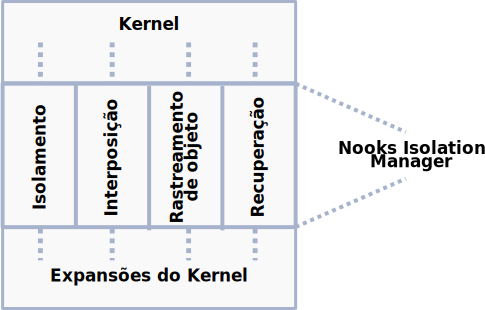
\includegraphics[width=0.8\textwidth]{nooks_nim}
	\caption[Visão geral da arquitetura do Nooks]{Visão geral da arquitetura do Nooks \citep{nooks}}
  \label{fig:nooks_nim}
\end{figure}

A Figura \ref{fig:nooks_nim} ilustra de forma geral a arquitetura de
\emph{Nooks}. Note que a comunicação entre o Kernel e as extensões (e vice-versa)
precisa passar pelo \emph{Nooks}. Esse intermédio é conduzido pelo \emph{Nooks
Isolation Manager (NIM)}, que é o responsável por implementar os objetivos do
projeto. \emph{Nooks} precisa estender-se em parte para o Kernel e em parte
para as extensões. No Kernel, é preciso alterar aquelas funções que são
disponibilizadas para as extensões ou que interagem com os módulos. Felizmente,
esse tipo de função pode ser detectado por algum padrão que, por sua vez, pode
ser abstraído para um \emph{script}. Além disso, esse tipo de modificação precisa ser
feito uma única vez. Do ponto de vista dos módulos, no geral, são poucos os
casos que precisam ser alterados diretamente, uma vez que eles fazem uso dos
recursos fornecidos pelo Kernel. Normalmente, módulos que exportam estruturas
de dados para o Kernel e o espaço de usuário também precisam ser alterados.

O \emph{Nooks} fornece isolamento por meio do LKPD: toda extensão
adicionada ao SO executa dentro do seu próprio LKPD que, por sua vez, é chamado
de \emph{contexto de execução}. Os domínios utilizam o mesmo nível de proteção
fornecido pelo processador para o Kernel, com a diferença de que o acesso de
escrita para certas porções é limitada e gerenciada pelo \emph{NIM}. Neste
sentido, podemos dividir o esquema de isolamento de \emph{Nooks} em duas partes:
o gerenciador de memória e o \emph{Extension Procedure Call} (XPC).

\begin{figure}[!h]
  \centering
  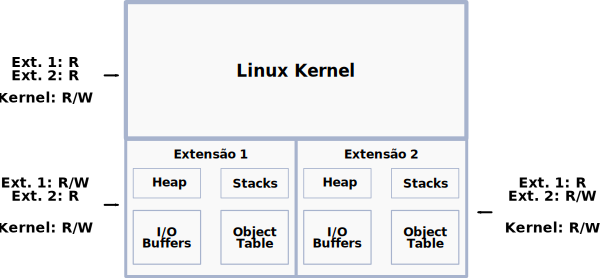
\includegraphics[width=0.8\textwidth]{nooks_mem}
  \caption[Acesso à memória do Nooks]{Acesso à memória do Nooks \citep{nooks}}
  \label{fig:nooks_mem}
\end{figure}

O gerenciador de memória de \emph{Nooks} é responsável por alocar, desalocar e
manipular os LKPDs. A Figura \ref{fig:nooks_mem} ilustra o \textit{kernel
address space}: note que o Kernel tem permissão de escrita e leitura sobre toda
a memória, mas os LKPDs mostrados só têm acesso de leitura e escrita a si mesmos.
A leitura de outras regiões de memória de dentro de um LKPD depende do controle
de acesso feito pelo NIM mas, no geral, só é permitida a leitura de outras
regiões da memória.

O outro mecanismo de isolamento fornecido pelo \emph{Nooks} é o XPC, que atua
como um serviço de transferência de controle criado para isolar as operações
feitas dentro do Kernel. A transferência de controle pode acontecer em duas
vias: do Kernel para a extensão (\texttt{nooks\_driver\_call}) e da extensão
para o Kernel (\texttt{nooks\_kernel\_call}). Essas funções esperam
três argumentos: um ponteiro para a função que será executada, uma lista de
argumentos e o domínio em que será executada. Toda vez que a rotina de
transferência é chamada, o contexto da pilha que realizou a chamada é salvo e o
\emph{Page Table} para o novo domínio alvo carregado.

Um dos objetivos do \emph{Nooks} é o de ser usado em SOs de produção. Para isso,
ele tem de se integrar com o SO de forma a causar o menor impacto possível
nas extensões. Por isso, \emph{Nooks} isola as extensões com XPC e também
implementa um mecanismo de rastreamento de estruturas de dados chamado
\emph{object-tracking} (parte do \emph{NIM}). O \emph{object-tracking} tem três
recursos básicos: (1) manter uma lista de estruturas de dados do Kernel que são
manipuladas por uma extensão, (2) controlar todas as modificações para essas
extensões e (3) fornecer informações de objetos para limpeza de dados quando a
extensão falhar. O rastreamento dos objetos começa com o armazenamento de todos
os objetos em uso por uma extensão e em seguida é feita uma associação entre o
Kernel e as versões das extensões.

Por fim, \emph{Nooks} possui um mecanismo de recuperação que busca detectar
falhas de software quando uma extensão é chamada de forma inapropriada ou se
uma extensão está consumindo muitos recursos. A estratégia de recuperação é
subdividida em duas partes: \emph{recovery management} e \emph{user-mode
agent}. O primeiro é responsável por desalocar recursos e, se necessário,
realocá-los. O segundo é quem coordena a ação de recuperação e
é definido no espaço de usuário. Note que a flexibilidade do \emph{agent-mode}
permite várias possíveis formas de recuperação, sendo a mais direta forçar a
remoção da extensão, seguida da reinserção e em seguida prosseguindo com a
execução da aplicação.

\emph{Nooks} utilizou uma base de dados de inserção de falhas em módulos para
validar a sua eficácia, conseguindo tratar 99\% dos casos. Além disso, os
autores também validaram o trabalho da perspectiva do desempenho e notaram que,
na maioria dos casos, os gastos com a estrutura são compensados pelas vantagens.

\section{Mondrian Memory Protection e Mondrix}

\citet{mmp} buscaram explorar técnicas para realizar controle fino sobre da
memória, com o objetivo de adicionar mais confiabilidade e segurança para os
SOs. Os autores discutem os problemas associados com a decisão usual de se promover
isolamento por meio da separação do espaço de endereçamento dos processos, que
por sua vez faz com que todas as \emph{threads} de um processo compartilhem um
mesmo domínio de proteção. Além disso, o modelo de paginação comumente adotado impõe um
tamanho fixo de página. Logo, o menor compartilhamento possível é o de uma página, que
tem o mesmo nível de permissão para todos os elementos contidos nela. Os autores
argumentam que, apesar das vantagem oferecidas pelo modelo atual, muitos
aspectos de segurança e estabilidade do sistema são comprometidos. Dois
exemplos são apontados pelos autores; o primeiro ilustra o caso do servidor
Apache, que pode carregar vários \textit{plugins} externos, contudo, se algum
código malicioso ou defeituoso for carregado ele comprometerá toda a
estabilidade do servidor (em alguns casos quebrando a aplicação). Outro exemplo
refere-se ao acesso de ponteiros em outros domínios da memória (por exemplo,
acesso do espaço de usuário para o do Kernel), que atualmente não são permitidos,
sendo necessário realizar operações de cópias.

\begin{figure}[!h]
  \centering
  \includegraphics[width=0.7\textwidth]{mondrix_pd}
	\caption[Representação dos domínios de proteção do Mondrix]{Representação dos domínios de proteção do Mondrix (\cite{mondrix})}
  \label{fig:mondrixPD} 
\end{figure}

Os autores defendem que mecanismos de controle fino do acesso à memória podem
trazer grandes benefícios em termos de segurança, confiabilidade e, em certos
casos, desempenho. Nesse sentido, \citet{mmp} propuseram uma abordagem
que permite o controle de acesso à memória no nível do tamanho das palavras de
dado. Para isso é apresentado um novo tipo de abordagem baseada em hardware e
software chamado \emph{Mondrian Memory Protection (MMP)}~\citep{mmp}. Além
disso, uma implementação prática chamada \emph{Mondrix}~\cite{mondrix} foi
feita no GNU/Linux. A Figura~\ref{fig:mondrixPD} resume a representação de
memória que o MMP busca atingir. Repare que não existem porções de memória
específica; a memória é dividida em diversos compartimentos chamados
\emph{Protection Domains (PD)}. Um PD é definido como um contexto que determina
a permissão para executar um código. Cada PD é independente do espaço de
endereçamento e pode conter múltiplas \emph{threads}, mas cada \emph{thread} só
pode pertencer a um único PD.  O projeto do MMP é guiado por três requisitos:

\begin{enumerate}
	\item \textbf{Diferente}: Cada PD diferente pode ter um domínio distinto
				para a mesma região de memória;
	\item \textbf{Pequeno}: A granularidade de compartilhamento deve ser menor
				do que uma página;
	\item \textbf{Revogável}: Um PD é dono da sua própria região de memória e
				pode mudar a forma como outros domínios veem a sua memória.
\end{enumerate}

% TODO: FIGURA K
Os autores afirmam que MMP tem a semântica da segmentação (Seção ~\ref{sec:segmentacao}) sem os problemas
associados a ela. MMP fornece controle fino sobre a proteção dos dados
compartilhados, utiliza endereçamento linear, é compatível com o conjunto de instruções
existentes, não necessita de registradores de segmentos, possui um mecanismo
simples de revogação de permissões e não tem ponteiros marcados. Para que
MMP possa garantir o controle de acesso à memória, ele precisa verificar as
permissões de acesso feitas por cada operação de \emph{load/store}; isto
claramente consome mais recursos computacionais. Por isso, MMP é uma solução
que também depende da utilização de um hardware personalizado.

% TODO: FIGURA G -> A princípio não me parece que falar do hardware é útil...
%\hltodo[A Figura G]{Segmentation Fault} ilustra a arquitetura de hardware proposta para a implementação do
%MMP; note que ela introduz muitos elementos novos. %TODO: Descrever o hardware

Da perspectiva do software, Mondrix \citep{mondrix} sugere a utilização de um
novo elemento chamado de Supervisor de Memória, dividido em duas partes:
uma parte superior, responsável pelo controle do acesso; e parte inferior, responsável
por escrever nas tabelas de permissão. A parte superior é a mais importante,
sendo responsável por manter e controlar as políticas, pela interface com o Kernel,
por rastrear objetos compartilhados e por implementar grupos de permissão. As
definições de permissão da memória são descritas por três elementos:

\begin{enumerate}
	\item \emph{Permissão de Acesso}: As permissões de acesso são definidas pelo
				seguinte conjunto de elementos: permissão do domínio, \emph{gates},
        tabela de pilha;
	\item \emph{Dono da Memória}: Define quem tem autoridade sobre a região de
				memória (domínio). Note que o espaço de endereçamento é contínuo e sem
				sobreposição, logo, cada região tem apenas um dono;
	\item \emph{Permissões Exportadas}: É possível exportar as permissões de
				acesso, permitindo que outras regiões chamem códigos
				fora do seu domínio. Contudo, a exportação pode ser controlada, de forma
				que outros trechos que acessem o código tenham uma visão limitada da
				região.
\end{enumerate}

Dados esses elementos, o Supervisor de Memória atua tomando as decisões
referentes ao acesso a uma dada região da memória.

Um aspecto interessante de se notar do Supervisor de Memória é a sua separação
lógica do alocador de memória. Mondrix permite que o Kernel escolha qual
alocador de memória deseja utilizar; isso é possível porque um domínio solicita
memória para o alocador e o Supervisor só estabelece as permissões para a
memória solicitada.
% Gosto muito dessa ideia de separar o alocador do controlador de acesso à
% memória, na minha opinião em termos práticas essa é uma das ideias mais
% valiosas desse trabalho.

O Supervisor também é responsável por revogar permissões quando uma região de
memória é liberada, além de manter o rastreamento de qual domínio tem acesso a
qual região de memória. O Supervisor ainda gerencia o acesso à pilha
das \emph{threads} (uma \emph{thread} só pode controlar pilha que estão
no seu domínio), cria e destrói proteções de domínio e também válida as
políticas de acesso.

\section{SpaceJMP}
\label{sec:mvas}

Toda vez que um processo é criado, ele inicializa diferentes estruturas de
dados relacionadas à sua execução. Um dos elementos fundamentais dos processos
é o espaço de endereçamento virtual (\emph{Virtual Address Space -- VAS}), que é
completamente acoplado aos processos. Normalmente, os VAS são maiores que a
memória física e são totalmente isolados de outros processos. Se um processo
precisar compartilhar dados com outros processos, será necessário criar e
gerenciar uma região de memória compatilhada que permita a escrita e/ou leitura
por outros processos. O atual modelo de VAS não dá suporte para
o compartilhamento de estruturas de dados entre processos com base em ponteiros;
normalmente, é necessário serializar os dados, o que tem se tornado um incômodo.

\begin{figure}[!h]
  \centering
  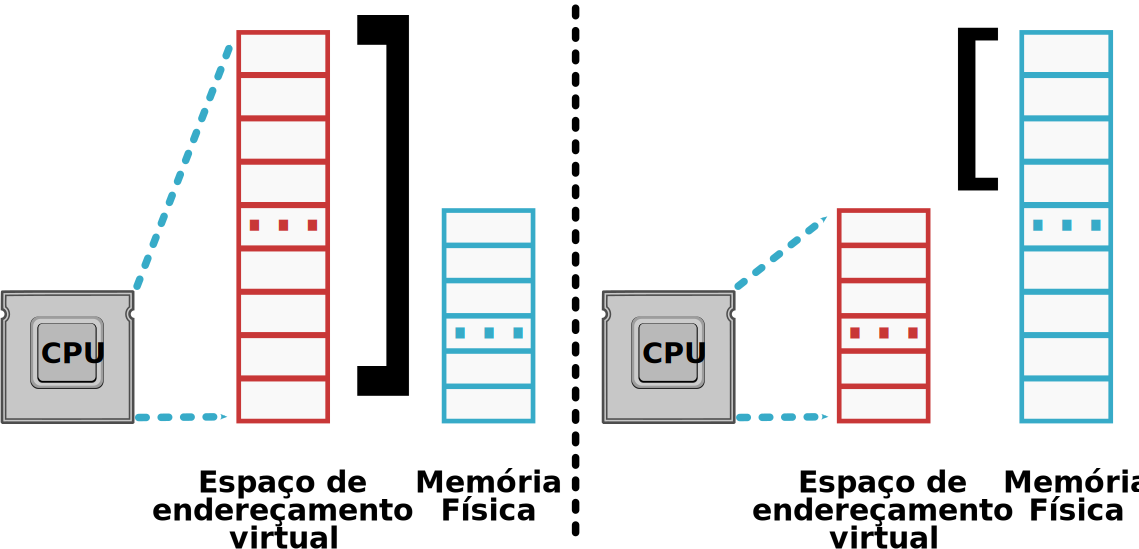
\includegraphics[width=.7\textwidth]{vas_vs_physical_address} 
  \caption{VAS e Memóra Física}
  \label{fig:vas_vs_physical} 
\end{figure}

No início dos anos 1990s, os processadores tinham poucos bits para o VAS, mas que eram suficientes
para endereçar toda a memória física disponível na época. Apesar disso, durante
esse período, o tamanho da memória cresceu consideravelmente e os processadores
não foram mais capazes de endereçar diretamente todo o endereço de memória disponível
\cite{crowley}. A Figura \ref{fig:vas_vs_physical} exemplifica o problema
mencionados acima: a parte da esquerda ilustra uma CPU com bits suficientes
para o VAS, que consegue endereçar todo o espaço de endereçamento
físico da memória. O lado direito da figura representa uma situação na qual o
VAS é menor do que a memória física. Assim, um um único processo não é capaz de
acessar toda a memória física disponível, impondo um limite ao processo
quanto ao tamanho que ele pode ter. Essa situação
não é uma novidade: enquanto a indústria não produzia
novos processadores com bits extras para elevar o tamanho da VAS, os
desenvolvedores tiveram que utilizar vários artifícios para superar o
problema de bits insuficientes. Hoje em dia, esse problema está sob controle,
uma vez que os processadores atuais possuem um grande espaço de endereçamento.
Contudo, estamos no início de uma geração da computação conhecida por
\emph{data-centric}, que será dominada por grandes memórias não-voláteis
\citep{outlook}. Assim, simplesmente incrementar o total de bits para o VAS nas
CPUs não sanará tão facilmente esse problema, pois elevar o número de bits na
VAS tem impactos na produção, desempenho e consumo de energia \citep{spacejmp}.

Um dos problemas do modelo de processos atual é a representação
das estruturas de dados baseadas em ponteiros fora dos
limites dos processos. A serialização de dados ou ponteiros especiais podem ser
empregados para resolver este problema, contudo, ambos os métodos são
incômodos, ineficientes e, em muitos casos, confusos \citep{spacejmp}. O segundo
problema está associado com a tarefa de coordenar o compartilhamento de memória
entre vários processos, uma vez que esta é uma tarefa complicada e tediosa.

Para tentar resolver os problemas citados, \citet{spacejmp} propuseram uma
técnica chamada \emph{SpaceJMP}. Os autores propõem desacoplar o VAS dos
processos e permitir que um único processo tenha Múltiplos VAS (MVAS)
associados a si. Nesse contexto, o VAS é promovido para um objeto de
primeira-classe no SO e dá ao processo a habilidade de gerir os muitos
VAS.

\begin{figure}[!h]
  \centering
  \includegraphics[width=.7\textwidth]{solve_huge_address_memory}
  \caption{Resolvendo o problema de endereçar memórias físicas grandes}
  \label{fig:large_memory}
\end{figure}

A Figura \ref{fig:large_memory} ilustra como MVAS resolve o problema de
endereçar memórias físicas maiores do que o VAS. Basicamente, todo processo
pode criar múltiplas VAS e alternar entre eles. Se os processos precisarem de
mais memória do que o disponível, basta criar um novo espaço de endereçamento
com o começo apontando para uma região de memória não utilizada e, em seguida,
anexar o novo VAS ao processo. O problema da serialização e compartilhamento de
dados também pode ser simplificado pelo MVAS: basta criar um VAS e permitir que
múltiplos processos se anexem a ele.

\begin{figure}[!h]
  \centering
  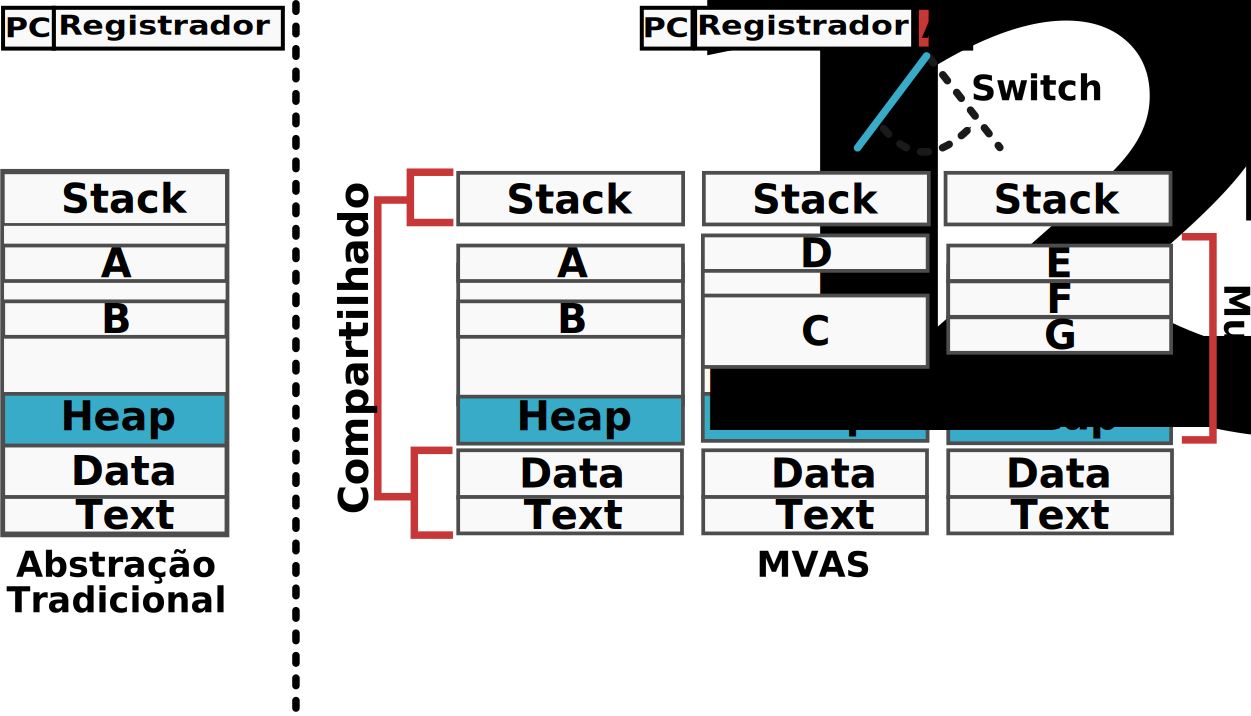
\includegraphics[width=.7\textwidth]{traditional_vs_mvas} 
	\caption[VAS e MVAS]{VAS e MVAS \citep{spacejmp}}
  \label{fig:traditional_vs_mvas} 
\end{figure}

A Figura \ref{fig:traditional_vs_mvas} ilustra a principal diferença entre um
processo com um VAS acoplado para um modelo no qual o VAS é desacoplado
(MVAS). O lado esquerdo da Figura mostra um processo tradicional, como explicado
na Seção \ref{sec:processos-e-threads}. O lado direito da figura representa um
processo com múltiplos VAS e diferentes informações dentro de cada \emph{Heap}
e segmentos de memória. Nesse novo cenário, a pilha, os dados e os segmentos
de texto são compartilhados entre os vários MVAS. Por fim, é importante
notar que os processos precisam manter a informação sobre o VAS atualmente em
execução.
 
Os autores da técnica fizeram uma implementação para GNU/Linux. A principal
funcionalidade do MVAS foi exposta para o usuário via \emph{system calls}. A
lista a seguir mostra o conjunto de funções expostas para o usuário:

\begin{itemize}
  \item \texttt{vas\_create()}: Cria um novo VAS com o nome indicado;
  \item \texttt{vas\_delete()}: Remove um VAS criado previamente;
  \item \texttt{vas\_find()}: Encontra um VAS de acordo com o nome;
  \item \texttt{vas\_attach()}: Anexa um VAS ao processo;
  \item \texttt{vas\_detach()}: Desanexa um VAS do processo;
  \item \texttt{vas\_switch()}: Muda o VAS atualmente instalado no processo para outro.
\end{itemize}

\begin{figure}[!h]
  \centering
  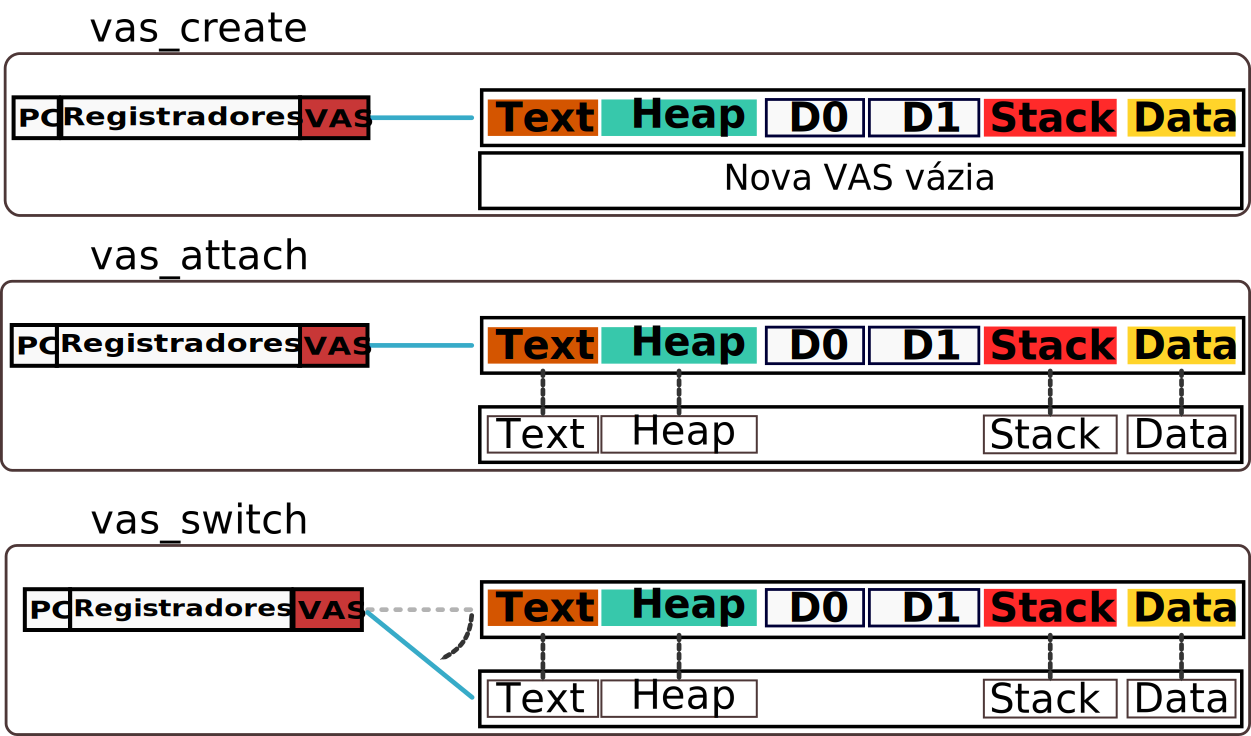
\includegraphics[width=.7\textwidth]{mvas_example} 
	\caption[System Call disponibilizada pelo SpaceJMP]{System Call disponibilizada pelo SpaceJMP \cite{ellarge}}
  \label{fig:mvas_example}
\end{figure}

A Figura \ref{fig:mvas_example} ilustra o comportamento das chamadas de sistema
implementadas. O topo da figura mostra um processo normal com um VAS padrão
associado a si; em seguida, a chamada para a função \texttt{vas\_create()} é
feita de forma a criar um novo VAS. Após a criação, é preciso anexar o VAS ao
processo por meio da chamada de sistema \texttt{vas\_attach()}. Por fim, o
processo pode mudar entre os VAS por meio da chamada para
\texttt{vas\_switch()}.

\section{Light-weight Contexts}
\label{sec:lwc}

O fluxo de execução do processo é controlado pelo \textit{Program Counter (PC)}
juntamente com os dados da memória. Por sua vez, o escalonador é a entidade que
orquestra quando retirar e inserir um novo processo para execução na CPU. Consequentemente,
tanto o PC quando os demais dados do processo são mantidos juntos no nível do
kernel.

\citet{litton} afirmam que o desacoplamento do isolamento da memória, estado de
execução e separação dos privilégios dos processos trazem benefícios. Com tal
ideia em mente, os atores sugerem uma nova abstração de processos chamada de
\textit{lightweight-context (lwC)}. Basicamente, cada processo pode ter um
(lwC root) ou mais lwCs, cada um com o seu próprio mapeamento
virtual da memória, descritor de arquivos e credenciais. Opcionalmente, a API
do lwC permite controlar quais elementos podem ser compartilháveis ou não entre
os lwCs.

Um lwC compreende um mapeamento de memória virtual, uma coleção de mapeamento
de páginas, \emph{bindings} de descritores de arquivos e conjuntos de
credenciais; sempre que um novo processo é criado, o sistema cria um novo lwC
para ele. A aplicação pode acessar todas as funcionalidades do lwC via espaço
do usuário através de chamadas de sistemas que fazem o controle fino dos
comportamentos fornecidos.

As chamadas mais interessantes são \texttt{lwCreate()} e \texttt{lwSwitch()}.
O \texttt{lwCreate()} tem uma semântica similar ao da chamada de sistema
\texttt{fork()}; assim que a chamada é feita, o processo pai tem os seus dados
duplicados no processo filho. Contudo, ao contrário do \texttt{fork()}, o
\texttt{lwCreate()} não cria uma nova \emph{thread} e nem um novo \emph{PID}.
Ao final da execução da chamada de sistema, o \texttt{lwCreate()} retorna um
identificador do novo contexto para o processo pai e se estiver no processo
filho ele retorna -1. A cópia do estado do processo pai na forma do contexto,
recebe o nome de \emph{snapshot}. Depois da criação do processo filho, a
aplicação é livre para fazer a troca (com o \texttt{lwSwitch()}) para algum de
seus \emph{snapshots} a qualquer momento.

A Figura \ref{fig:lwc} ilustra a operação de troca entre diferentes lwCs. Um
processo pode criar vários lwCs durante a sua execução e em
diferentes momentos e pode
seletivamente escolher transferir o seu fluxo de execução para outro lwC por
meio de uma chamada para \texttt{lwSwitch()}. A mudança da \emph{thread} é
feita pelo SO, que é responsável por mudar automaticamente o mapeamento da
memória virtual, as entradas das tabelas de arquivos, o PC e o \emph{stack
pointer}.

\begin{figure}[!h]
  \centering
  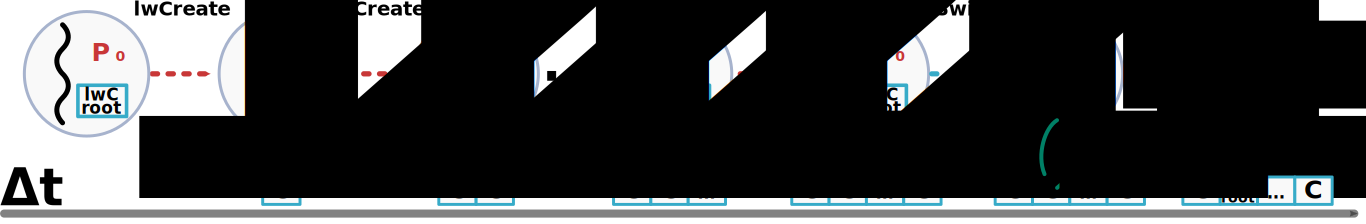
\includegraphics[width=\textwidth]{lwC} 
  \caption{Exemplo do comportamento do lwC}
  \label{fig:lwc} 
\end{figure}

A interface de lwC também permite que outras operações, como compartilhamento
dinâmico ou estático de recursos, controle sobre o acesso as
\emph{capabilities}, emulação de chamadas de sistema e novas camadas de
isolamento dentro do processo. Todo o conjunto de chamadas de sistema do lwC
fornece um sofisticado modelo de programação que permite novas capacidades
tais quais rápido \emph{roll-back}, isolamento de seções e compartimentos de
proteção. A API do lwC é composta das seguintes funções:

\begin{itemize}
  \item \texttt{lwCreate(resource-spec,options):} Cria um novo contexto de acordo com o estado atual do processo;
  \item \texttt{lwSwitch(target, args):} Alterna entre os diferentes contextos;
  \item \texttt{lwRestrict(l, resource-spec):} Permite restringir a forma de acesso ao contexto;
  \item \texttt{lwSyscall(target, mask, syscall, syscall-args):} Intercepta chamadas de sistema dentro de um contexto permitindo validar permissões de execução.
\end{itemize}

Os autores demonstram os conceitos do lwC em uma implementação no FreeBSD. As
modificações principais foram feitas no gerenciador de memória e estruturas de dados do
processo. Seu uso foi demonstrado em adaptações feitas no Apache, Nginx e
OpenSSH. Por fim, os autores propõem certos algoritmos que discutiremos no
Capítulo \ref{cap:analise-sobre-abstracoes-de-processos}.

\section{Exokernel}
\label{sec:exokernel}

\citet{exokernel} defendem que os projetos de SOs possuem uma série de
desvantagens por terem várias abstrações diretamente programadas no núcleo. Os
autores argumentam que as abstrações implementadas diretamente no SO possuem
sérios impactos no desempenho, reduz consideravelmente a flexibilidade das
aplicações e limita as possibilidades de ampliar as funcionalidade
disponibilizadas no espaço do usuário. A implementação dessas abstrações
diretamente no núcleo do SO são problemática uma vez que: impedem a aplicação
de tirar proveito das otimizações que são especificas do seu domínio, as
mudanças em tais abstrações são desencorajadas e reduzem as possibilidade do
que pode ser feito no espaço de usuário.

Segundo os autores, a fixação das abstrações de alto-nível apresentam as
seguintes limitações:

\begin{itemize}
  \item A degradação do desempenho ocorre uma vez que atender ao maior número
        de aplicações possível com a mesma abstração tem um custo
        computacional. Por exemplo, algumas aplicações podem sofrer com o
        \emph{overhead} gerado por outras camadas de abstrações na qual não
        precisa;
  \item As informações de utilização de recursos são escondidas das aplicações,
        isto dificulta a aplicação ter controle sobre os recursos utilizados;
  \item As aplicações ficam limitadas a utilizar apenas aquelas interfaces
        padrão fornecidas pelo SO.
\end{itemize}

Por fim, com esses problemas em mente e motivados pela antiga observação de que:
quanto mais baixo o nível das primitivas (simples), mais eficientemente ela
pode ser implementada e maior a amplitude de ação fornecida para abstrações de
alto-nível; os autores propuseram uma nova arquitetura de SO chamada
\emph{exokernel}.

\emph{Exokernel} busca ser um núcleo mínimo que permita multiplexar de forma
segura os recursos de hardware e ao mesmo tempo fornecer uma interface de
baixo-nível na qual as abstrações do SO podem ser construída sobre ela. Para
que seja possível implementar um SO usando este conceito é preciso implementar
a chamada \textit{biblioteca do SO} com acesso aos recursos de baixo nível e
com as abstrações construídas nela (p.ex. processos, arquivos, escalonador,
etc). Para que a implementação de tal conceito seja possível, os autores os
seguintes princípios:

\begin{enumerate}
  \item \textbf{\emph{Expor o hardware de forma segura:}} O conceito
        fundamental do \emph{exokernel} consistem em exportar de forma segura
        e controlada o acesso de baixo nível ao hardware, por isto toda
        implementação do \emph{exokernel} deve concentrar-se em exportar os
        privilégios e recursos de máquina. Por isto ele não deve impor
        abstrações de alto-nível, i.e, o \emph{exokernel} deve evitar gerir
        recursos;
  \item \textbf{\emph{Expor alocações:}} Um \emph{exokernel} deve permitir que
        uma biblioteca de SO aloque recursos. Além disto, os recursos não devem
        ser implicitamente alocados uma vez que a biblioteca de SO tem a
        obrigação de participar de todas as decisões de alocação;
  \item \textbf{\emph{Expor nomes:}} Um \emph{exokernel} deve exportar nomes
        físicos. Isto é eficiente uma vez que reduz o nível de indireção, e por
        sua vez o número de traduções necessárias entre nomes virtuais e
        físicos. Por fim expor nomes físicos também encapsula atributos de
        recursos uteis, por exemplo, um sistema de caches fisicamente indexado
        e diretamente mapeado, tem o nome da página física (i.e. o número da
        página) determina qual página que conflita;
  \item \textbf{\emph{Expor revogações:}} Um \emph{exokernel} deve utilizar um
        protocolo de revogação de recursos explicitas para que a biblioteca do
        SO possa gerir os recursos de forma eficiente;
\end{enumerate}

Por fim, além desses princípios o \emph{exokernel} também deve especificar as
políticas para arbitrar a competição entre as bibliotecas do SO. Dado esses
princípios o \emph{exokernel} deve disponibilizar as seguinte tarefas: ligação
segura, visibilidade de recursos e protocolo de falha.

A ligação segura (\emph{Secure Bindings - SB}) é o mecanismo que desacopla a
autorização do uso dos recursos. Para implementar o SB é preciso um conjunto de
primitivas que a aplicação pode usar para expressar verificações de proteção.
Essas podem ser implementadas em hardware ou software, por exemplo, a entrada
da TLB é uma primitiva de hardware. Na prática o SB trabalha com o conceito de
"baixar o código para o kernel", esse código é chamado para cada acesso ou
evento do recurso para determinar o dono e a ação que o Kernel deve tomar.
Baixar o código dentro do kernel permite uma \emph{thread} da aplicação ter controle
sobre os eventos. Isto melhora o desempenho uma vez que elimina a camada
intermediaria do Kernel e também propícia limitar a aplicação aos seus
recursos.

A tarefa de \emph{revogação visível} é o mecanismo para recuperar os recursos
e romper com o SB estabelecidas. Vale observar que este mecanismo pode ser
visível ou invisível para a aplicação. Tradicionalmente os SOs realizam a
revogação de forma invisível desalocando recursos sem o envolvimento da
aplicação. O \emph{exokernel} utiliza revogação visível para a maioria dos
recursos, mesmo o processador é explicitamente revogado ao fim de um tempo de
execução determinado de forma que a biblioteca do SO é informada para que possa
reagir. O processo de revogação é como um diálogo entre o \emph{exokernel} e a
biblioteca do SO; a biblioteca precisa organizar uma lista de recursos que pode
ser desalocado rapidamente.

Por fim, um \emph{exokernel} pode definir um segundo estágio de revogação no
seu protocolo, na qual um pedido se torna um imperativo. Isto ajuda no caso em
que a biblioteca do SO falha, então o \emph{exokernel} pode simplesmente
quebrar o SB e informar a biblioteca. Todos as perdas de recursos forçadas são
armazenadas em um vetor de recuperação.

% \subsection{Singularity}
% 
% \subsection{Corey}

\section{Considerações Finais}

Neste capítulo buscamos apresentar diversos trabalhos que representam
contribuições variadas para a áreas da abstração de processos. Durante essa
pesquisa, vários trabalhos foram analisados, contudo por uma questão prática
selecionamos aqueles que trazem propostas diferentes e que podem ser
combinadas. No próximo capítulo, faremos uma análise sobre validações de tais
trabalhos.
